\documentclass{article}
% these lines load any packages you might wish to use. 
% some common ones are loaded below
\usepackage{amsfonts, amsmath, amssymb}
\usepackage[numbers,square,sort&compress]{natbib}
\usepackage{graphicx}  % required for inserting images
\usepackage{hyperref}  % for inserting urls, and having clickable links to equation and figure numbers
\usepackage[margin=1.2 in]{geometry}  % these margins are easy to read
\geometry{letterpaper}                   % ... or a4paper or a5paper or ... 
\usepackage{lmodern}		% good font
\usepackage{float}
\usepackage{graphicx}
\usepackage{subcaption}

\usepackage{tikz}  % for using tikz, to draw your own figures
\usetikzlibrary{angles,quotes}

% input document information here
\title{Fountain Trajectory Modelling Under Wind and Drag}
\author{Pavitra Bhargavi Allamaraju (90215237), Serena Khatwa (59879775), Tia Tia (41266891)}
%\date{}  % if you uncomment this, it will not put the date.
%\date{Dec 99, 1999}   % if you uncomment this, it will list the date as whatever is inside the curly brackets


\begin{document}

\maketitle

\section{Introduction}

Urban outdoor fountains create visual patterns by ejecting pressurized water jets from fixed nozzles into the air. The resulting jet trajectories are designed to achieve a prescribed height and to land within a bounded fountain basin, ensuring aesthetic consistency while minimizing water loss and overspray. In real world conditions, however, environmental disturbances, particularly wind, can significantly alter the jet trajectory. Wind introduces aerodynamic forces that bend the jet, shift its landing location, and reduce the reliability of the intended fountain pattern.

From a design perspective, fountain performance depends on the interplay between nozzle orientation, aerodynamic drag, and ambient wind conditions. While nozzle exit speed is often constrained by mechanical and operational considerations, parameters such as launch angle and effective drag may vary, and wind speed can change unpredictably. Understanding how these factors influence jet trajectories is therefore essential for determining geometric design requirements, such as the minimum basin radius needed to ensure robust operation \cite{wang2024centrifugal}.

The goal of this project is to develop a deterministic mathematical model for the motion of a water jet using ordinary differential equations that incorporate gravity, aerodynamic drag and wind velocities. The nozzle exit speed is treated as fixed, while wind speed, drag strength and launch angle are varied systematically. By analyzing how these parameters affect the jet’s trajectory and landing location, we identify the minimum basin radius required to contain the jet under a range of wind conditions. This approach reframes wind robustness as a geometric design problem and provides quantitative guidance for fountain basin sizing based on environmental constraints.

\section{Model}

We adopt a deterministic modelling approach to study the motion of an outdoor fountain jet under environmental disturbances. The model is governed by principles of classical mechanics including Newton’s Second Law and quadratic aerodynamic drag \cite{lubarda2022review}. To enable systematic analysis and comparison across parameter regimes, the governing equations are nondimensionalized and solved numerically, and the resulting trajectories are used to predict the minimum basin radius required for wind-robust operation.

\subsection{Assumptions}

We model the water jet as an effective point mass, or representative water parcel, whose motion captures the overall water trajectory. The mass off this parcel is assumed to remain constant during its flight, and effects such as evaporation, breakup, and phase change are neglected. We assume the water is emitted from a fixed nozzle with a constant exit speed and fixed launch angles throughout a single trajectory, corresponding to steady operating conditions. The jet motion is governed solely by gravity and aerodynamic drag, with wind represented as a prescribed velocity field that remains steady during the jet’s flight, and all other atmospheric conditions are assumed constant. The fountain basin is circular with a fixed radius, and we consider a trajectory acceptable only if the jet lands within this boundary. The nozzle is positioned at the center of the basin, and the fountain layout exhibits five-fold rotational symmetry, dividing the basin into five identical angular sectors. Owing to this symmetry, we analyze the jet trajectory within a single sector and obtain the remaining nozzle trajectories by rotation. Finally, interactions between different water jets are neglected, and each jet is assumed to evolve independently.



\subsection{Construction}

We construct a mathematical model for the motion of a fountain jet using Newton’s second law, treating the jet as a point mass subject to gravity and aerodynamic drag. Let
$\mathbf{r}(t) = (x(t), y(t), z(t))$
denote the position of the jet at time \(t\), and let
$\mathbf{v}(t) = \dot{\mathbf{r}}(t)$
be its velocity. The jet is emitted from a fixed nozzle at the origin with constant exit speed \(v_0\), launch angle \(\theta\), and azimuthal angle \(\phi\).

Two forces act on the jet during its flight: gravity and aerodynamic drag. Gravity acts vertically downward with constant acceleration \(g\), giving the force \cite{FitzpatrickProjectileDrag}
\[
\mathbf{F}_{\text{grav}} = - m g \,\hat{\mathbf{z}},
\]
where \(m\) is the effective mass of the representative water parcel.

To incorporate wind effects, we define the relative velocity between the jet and the surrounding air as $\mathbf{v}_{\mathrm{rel}} = \mathbf{v} - \mathbf{u}_w,$ where \(\mathbf{u}_w\) is the prescribed wind velocity vector. Aerodynamic drag is modeled as a quadratic force opposing the relative motion, which is appropriate for high-Reynolds-number flow \cite{lubarda2022review, wang2024centrifugal}. The standard drag law gives
\[
\mathbf{F}_{\text{drag}}
= - \frac{1}{2}\rho_a C_d A
\lVert \mathbf{v}_{\mathrm{rel}} \rVert
\mathbf{v}_{\mathrm{rel}},
\]
where \(\rho_a\) is the air density, \(C_d\) is the drag coefficient, and \(A\) is the effective cross-sectional area of the jet \cite{LumenDragForces}.

Dividing by the mass \(m\), the drag acceleration becomes
\[
\mathbf{a}_{\text{drag}}
= - k \lVert \mathbf{v} - \mathbf{u}_w \rVert (\mathbf{v} - \mathbf{u}_w),
\qquad
k = \frac{\rho_a C_d A}{2m}.
\]
The parameter \(k\) therefore represents an effective drag strength that combines all physical properties related to aerodynamic resistance.

A summary of the variables and parameters are provided in Table 1 and Table 2.

\begin{table}[H]
\centering
\renewcommand{\arraystretch}{1.3}
\begin{tabular}{c|l|l|c}
Symbol & Description & Type & Dimensions \\
\hline
$t$ & time & independent variable & $[T]$ \\
$x$ & horizontal position (E--W) & dependent variable & $[L]$ \\
$y$ & horizontal position (N--S) & dependent variable & $[L]$ \\
$z$ & vertical position & dependent variable & $[L]$ \\
$v_x$ & horizontal velocity in $x$-direction & dependent variable & $[LT^{-1}]$ \\
$v_y$ & horizontal velocity in $y$-direction & dependent variable & $[LT^{-1}]$ \\
$v_z$ & vertical velocity & dependent variable & $[LT^{-1}]$ \\
$v_0$ & nozzle exit speed & parameter (fixed) & $[LT^{-1}]$ \\
$\theta$ & launch (elevation) angle of nozzle & parameter & $1$ \\
\end{tabular}
\caption{State variables and nozzle parameters}
\end{table}

\begin{table}[H]
\centering
\renewcommand{\arraystretch}{1.3}
\begin{tabular}{c|l|l|c}
Symbol & Description & Type & Dimensions \\
\hline
$\phi$ & azimuth angle of nozzle & parameter & $1$ \\
$\mathbf{u}_w = (u_x,u_y,u_z)$ & wind velocity vector & parameter & $[LT^{-1}]$ \\
$g$ & acceleration due to gravity & parameter & $[LT^{-2}]$ \\
$\rho_a$ & density of air & parameter & $[ML^{-3}]$ \\
$\rho_w$ & density of water & parameter & $[ML^{-3}]$ \\
$C_d$ & drag coefficient & parameter & $1$ \\
$A$ & effective cross-sectional area of jet & parameter & $[L^2]$ \\
$m$ & mass of water parcel & parameter & $[M]$ \\
$R$ & radius of fountain basin & parameter & $[L]$ \\
$k = \dfrac{\rho_a C_d A}{2m}$ & effective drag strength & parameter & $[L^{-1}]$ \\
\end{tabular}
\caption{Environmental and physical parameters used in the model}
\end{table}


\subsection{Governing Equations}

Applying Newton’s second law, the equations of motion for the jet are \cite{FitzpatrickProjectileDrag}
\[
\frac{d\mathbf{r}}{dt} = \mathbf{v},
\ \ \ \ \ \ 
\frac{d\mathbf{v}}{dt}
= - g\,\hat{\mathbf{z}}
- k \lVert \mathbf{v} - \mathbf{u}_w \rVert (\mathbf{v} - \mathbf{u}_w).
\]
This system of ordinary differential equations is deterministic: for given initial conditions and parameter values, the jet trajectory is uniquely determined.

The initial conditions corresponding to the nozzle settings are \cite{peszynski2019mathematical}

\[
\mathbf{r}(0) = (0,0,0), \qquad
\mathbf{v}(0) = v_0
\begin{pmatrix}
\cos\theta \cos\phi \\
\cos\theta \sin\phi \\
\sin\theta
\end{pmatrix}.
\]

\subsection{Nondimensionalized System of Equations}

To reduce the number of parameters and clarify the relative importance of physical effects, we nondimensionalize the governing equations \cite{WallsDanielsProjectile2022}. We choose the basin radius \(R\) as the characteristic length scale and the nozzle exit speed \(v_0\) as the characteristic velocity scale, giving the time scale $T = \frac{R}{v_0}.$

We define nondimensional variables
\[
\mathbf{r} = R \mathbf{r}^*, \qquad
\mathbf{v} = v_0 \mathbf{v}^*, \qquad
t = T \tau, \qquad
\mathbf{u}_w = v_0 \mathbf{u}^*.
\]

Substituting these scalings into the governing equations yields
\[
\frac{d\mathbf{r}^*}{d\tau} = \mathbf{v}^*,
\ \ \ \ \ \ 
\frac{d\mathbf{v}^*}{d\tau}
= - \Gamma \hat{\mathbf{z}}
- \Lambda \lVert \mathbf{v}^* - \mathbf{u}^* \rVert (\mathbf{v}^* - \mathbf{u}^*),
\]
where the dimensionless parameters
\[
\Gamma = \frac{gR}{v_0^2}, \qquad
\Lambda = kR
\]
measure the relative influence of gravity and aerodynamic drag, respectively.

\subsection{Landing Condition}

The jet trajectory is integrated until it reaches the ground plane,
$z^*(\tau_L) = 0, \qquad v_z^*(\tau_L) < 0.$
The horizontal landing location \((x_L^*, y_L^*)\) determines the landing radius
\[
r_L^* = \sqrt{x_L^{*2} + y_L^{*2}},
\]
which represents the minimum basin radius, relative to \(R\), required to contain the jet under the given wind and nozzle parameters.

\subsection{Symmetry Considerations}
The fountain design consists of five identical nozzles arranged symmetrically about the basin center. Due to the rotational symmetry of the geometry and governing equations, nozzle directions differ only by a rotation of $\frac{2\pi}{5}$ in the azimuthal angle $\phi$. Consequently, it is sufficient to model and analyze the trajectory of a single nozzle; the behavior of the remaining nozzles follows directly by symmetry as shown in Figure 1.




\begin{figure} [H]
    \centering
    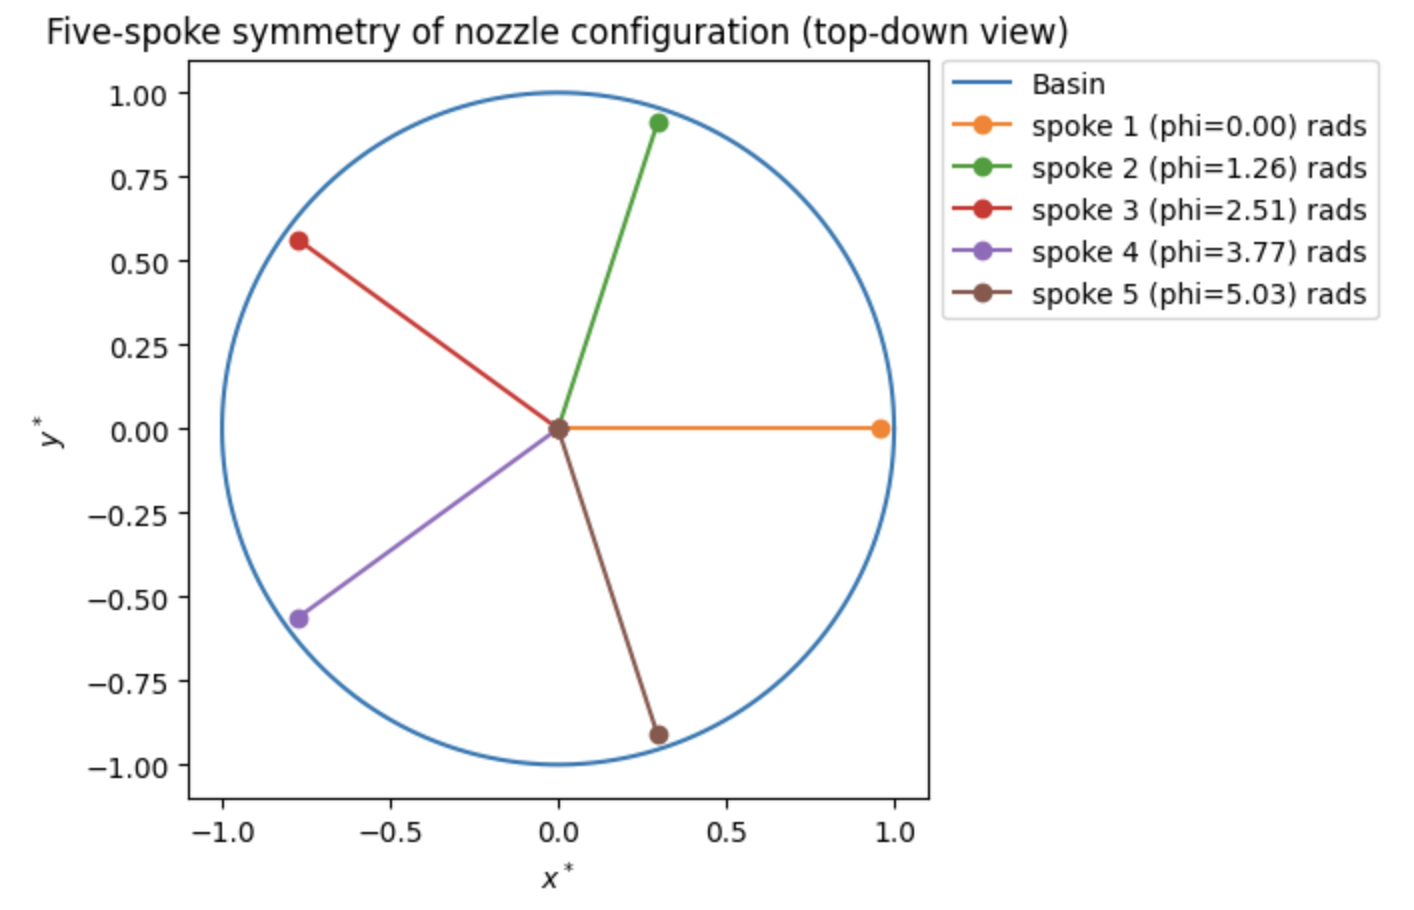
\includegraphics[width=0.5\linewidth]{Figure0.png}
    \caption{Five-Spoke Symmetry of Nozzle Configuration}
    \label{fig:placeholder}
\end{figure}




%\begin{figure}
%\centering
%\begin{tikzpicture}
% Define the radius of the discs
%\def\cth{0.14231483827}%{0.2588190451}
%\def\sth{0.98982144188 }%{0.96592582628}
%\def\rad{0.7}
%\def\radb{0.4}
% Define the parallelogram vertices (centers of the discs)
% The discs touch each other, so distance between centers = 2*radius
%\coordinate (A) at (0, 0);
%\coordinate (B) at (2*\rad, 0);
%\coordinate (C) at (2*\rad + 2*\rad*\cth, 2*\rad*\sth);
%\coordinate (D) at (2*\rad*\cth, 2*\rad*\sth);
% Draw the four discs
%\fill[blue!20, draw=black, thick] (A) circle (\radb);
%\fill[blue!20, draw=black, thick] (B) circle (\radb);
%\fill[blue!20, draw=black, thick] (C) circle (\radb);
%\fill[blue!20, draw=black, thick] (D) circle (\radb);
% Draw the connecting lines between centers
%\draw[thick, black] (A) -- (B);
%\draw[thick, black] (B) -- (C);
%\draw[thick, black] (C) -- (D);
%\draw[thick, black] (D) -- (A);
% Mark the centers
%\fill (A) circle (2pt);
%\fill (B) circle (2pt);
%\fill (C) circle (2pt);
%\fill (D) circle (2pt);
% Optional: Label the centers
%\node[left] at (A) {$a$};
%\node[right] at (B) {$b$};
%\node[right] at (C) {$c$};
%\node[left] at (D) {$d$};
% Draw the angle at A with dotted lines
%\draw pic[draw, dotted, thick, angle radius=0.6cm, angle eccentricity=1.3, "$\theta$"] {angle = B--A--D};
%\end{tikzpicture}
%    \caption{The figure caption should explain the ingredients of the figure. The figure should have large enough fonts and marker sizes. Usually this means changing the defaults in matplotlib. See Figure \ref{fig:example} for an example of all of this.}\label{fig:awesomefigure}
%\end{figure}


\section{Results}

The nondimensional ODE system was solved numerically using standard time-stepping methods until the jet reached the ground plane. The landing location was recorded for varying wind strengths and nozzle parameters, and the results were analyzed in terms of trajectory shape, landing position, and sensitivity to design choices.

\subsection{Effect of Launch Angle on Jet Trajectories}

Plotting landing radius vs. launch angle for each spoke reveals that a launch angle of greater than $18$ degrees or less than $69$ degrees satisfies the requirement that fountain jet trajectories must land within the basin boundary. The landing range increases as launch angle increases from $0$ to $45$ degrees, and is maximized at $45$ degrees. The landing range decreases again as launch angle increases from $45$ to $90$ degrees, as expected based on ideal projectile motion. Based on the findings of these plots, we set the launch angle to $75$ degrees, as this retains the water trajectory within the fountain basin.


\begin{figure}[H] 
    \centering
    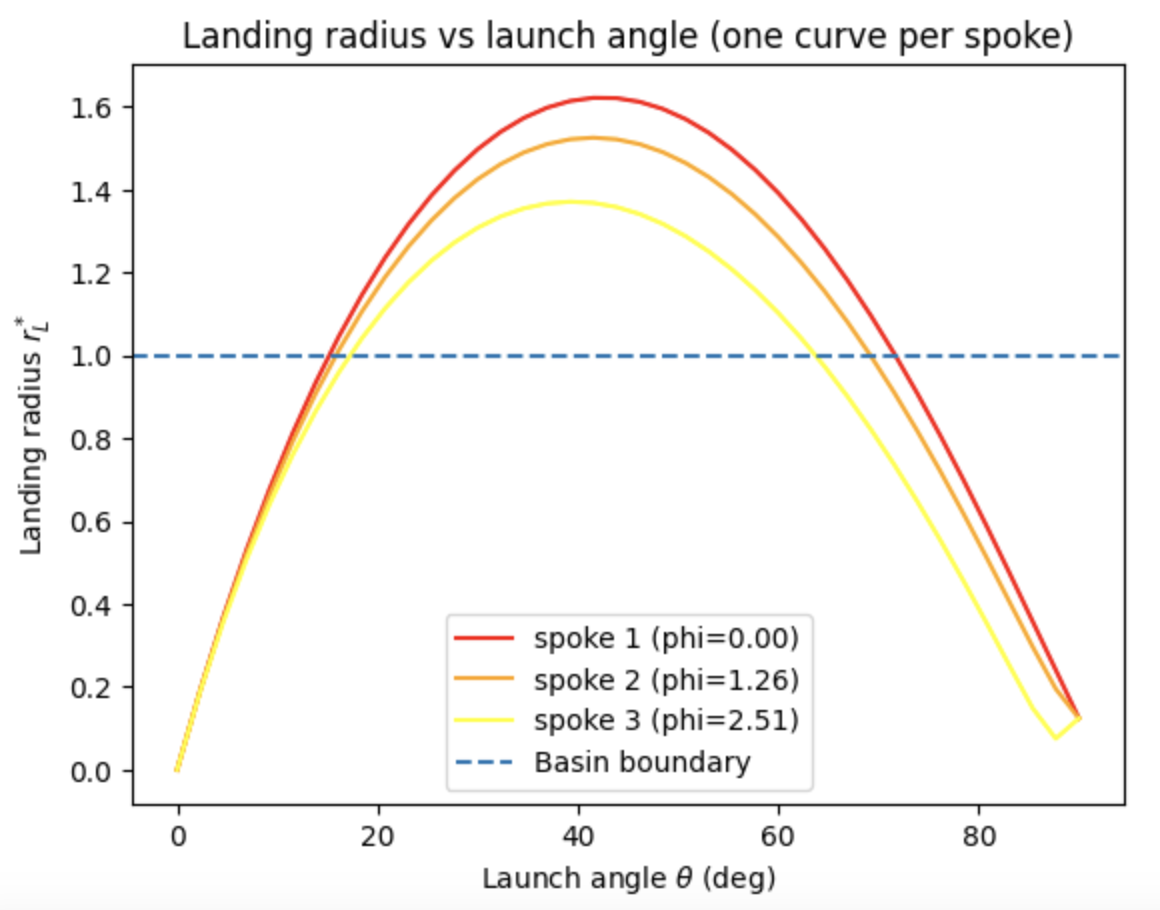
\includegraphics[width=0.37\textwidth]{Figure6.png}
    \hspace{0.5cm}
    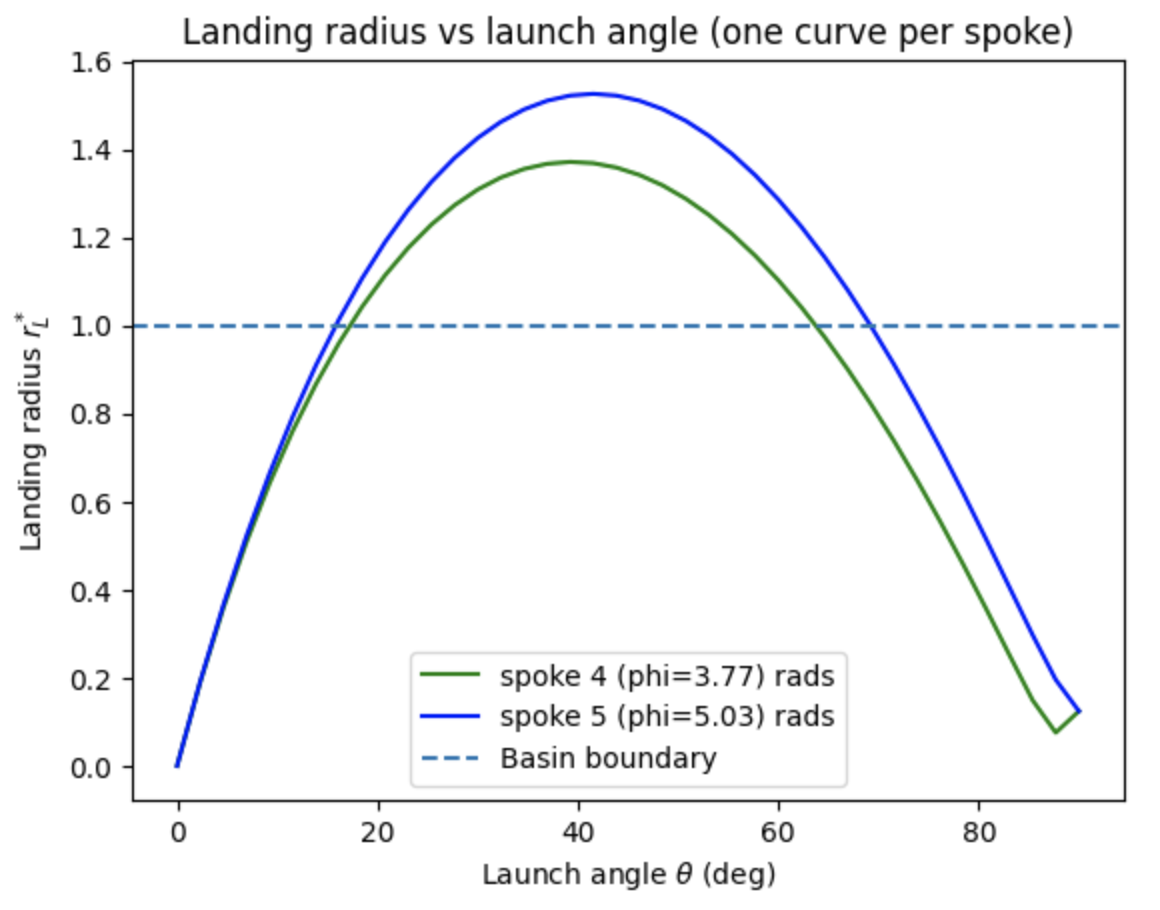
\includegraphics[width=0.37\textwidth]{Figure7.png}
    \caption{Landing Radius vs. Launch Angle}
\end{figure}

%\begin{figure} [H]
%    \centering
%    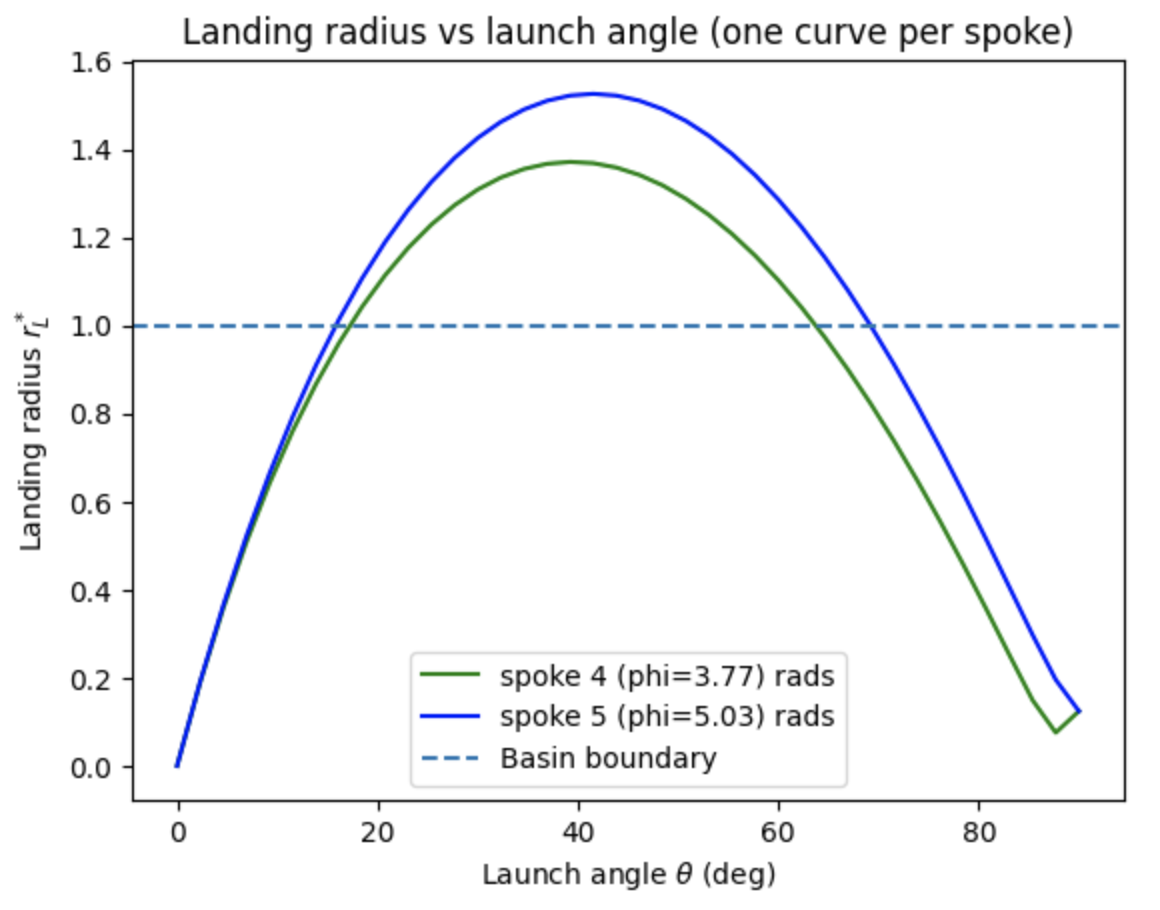
\includegraphics[width=0.5\linewidth]{Figure7.png}
%    \caption{Landing Radius vs. Launch Angle}
%    \label{fig:placeholder}
%\end{figure}

%\begin{figure} [H]
%    \centering
%    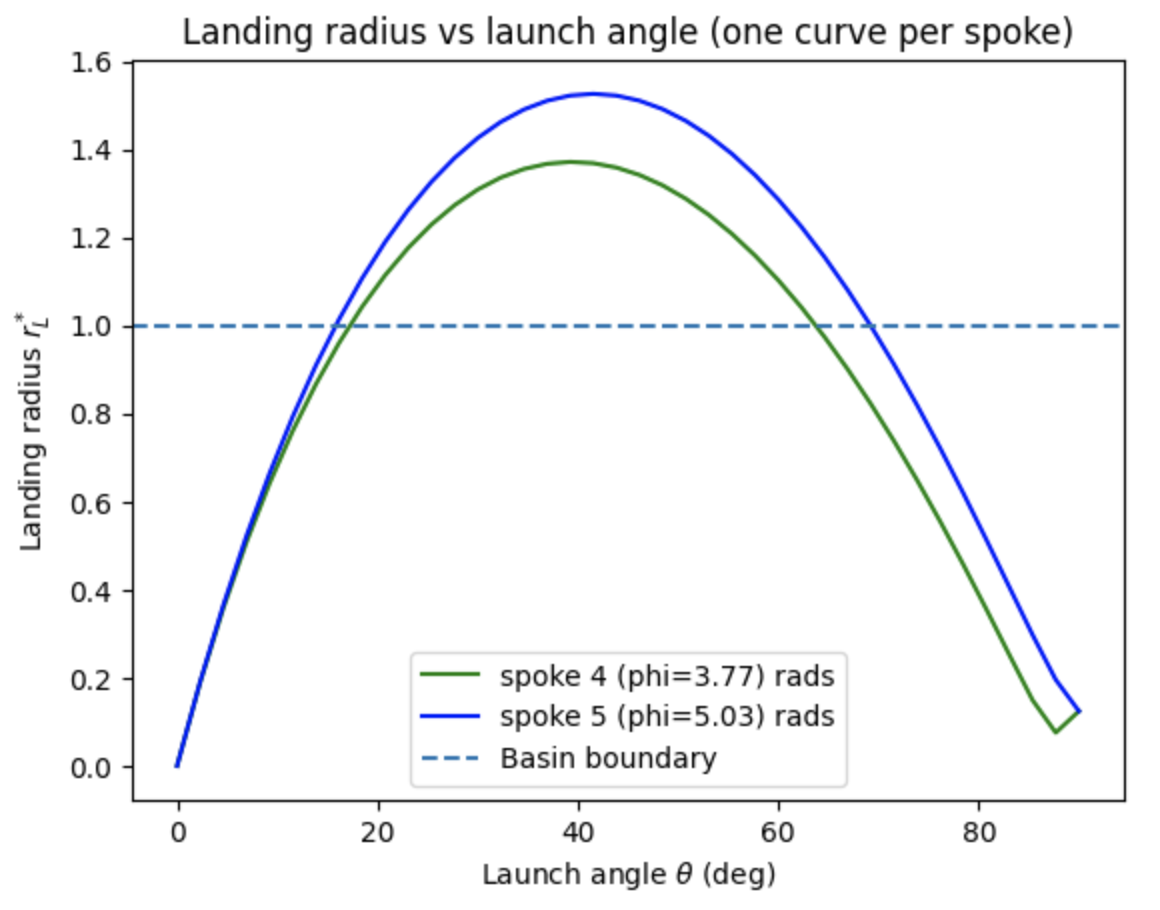
\includegraphics[width=0.5\linewidth]{Figure7.png}
%    \caption{Landing Radius vs. Launch Angle}
%    \label{fig:placeholder}
%\end{figure}

\subsection{Effect of Drag on Jet Trajectories}

Once the optimal launch angle is set to $75$ degrees, we investigate the effects of drag on the fountain trajectories. Plotting drag strength vs. landing reveals that a small amount of drag is necessary in order for the fountain trajectories to land within the basin.

\begin{figure}[H]
    \centering
    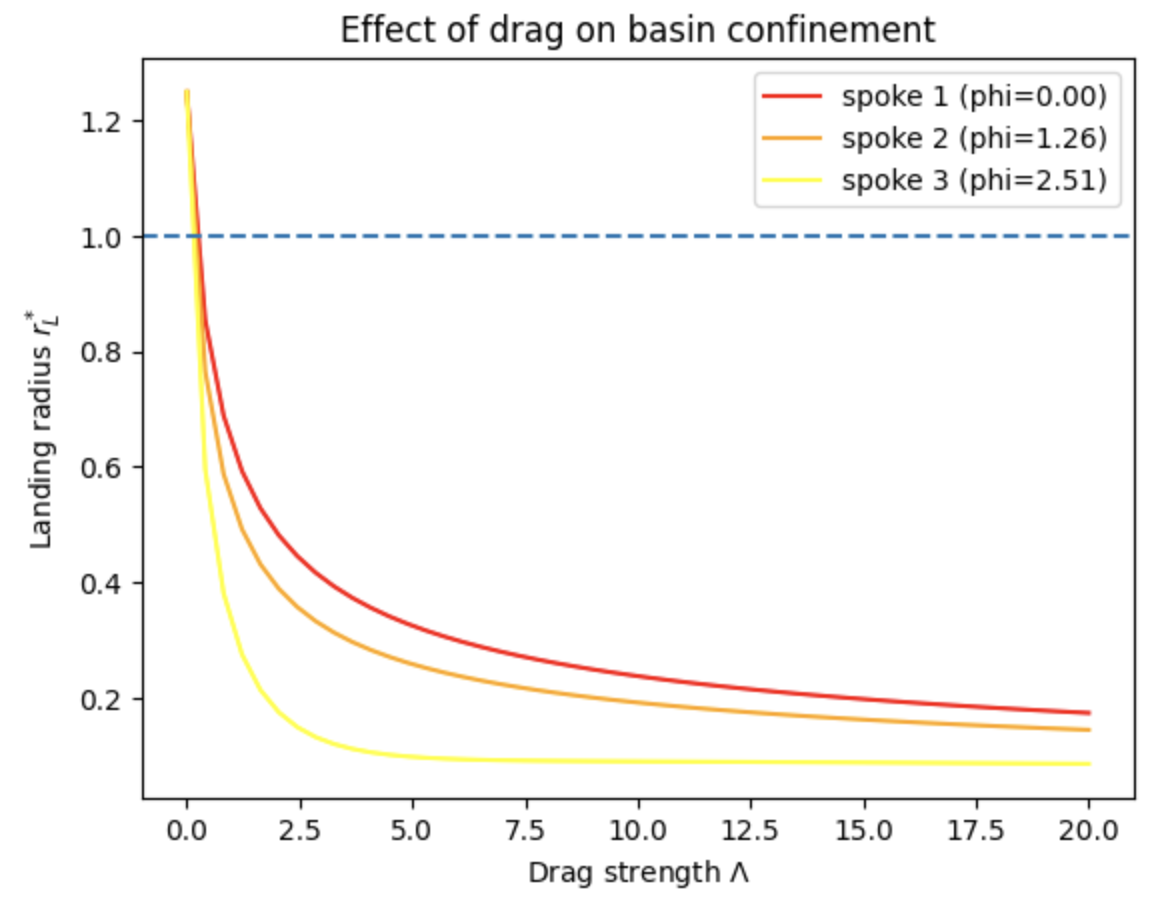
\includegraphics[width=0.37\textwidth]{Figure9.png}
    \hspace{0.5cm}
    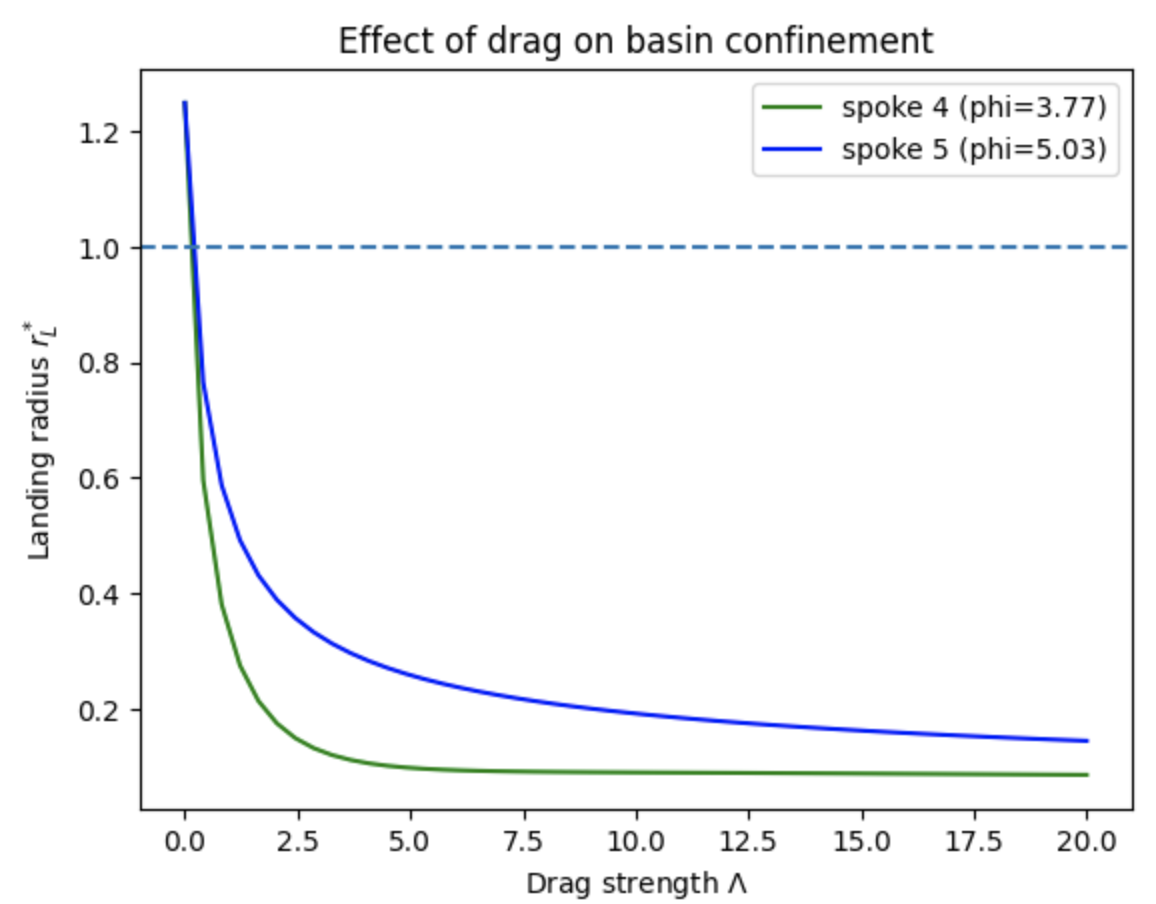
\includegraphics[width=0.37\textwidth]{Figure10.png}
    \caption{Effect of Drag on Basin Confinement}
\end{figure}
Visualizing the 3D trajectories under various drag strengths reveals that we must set the drag parameter lambda to at least 0.5, as setting 0 drag leads to the overspray of the water trajectory beyond the basin boundary. We can also see the height decreasing slightly on the vertical axis as drag increases.

\begin{figure} [H]
    \centering
    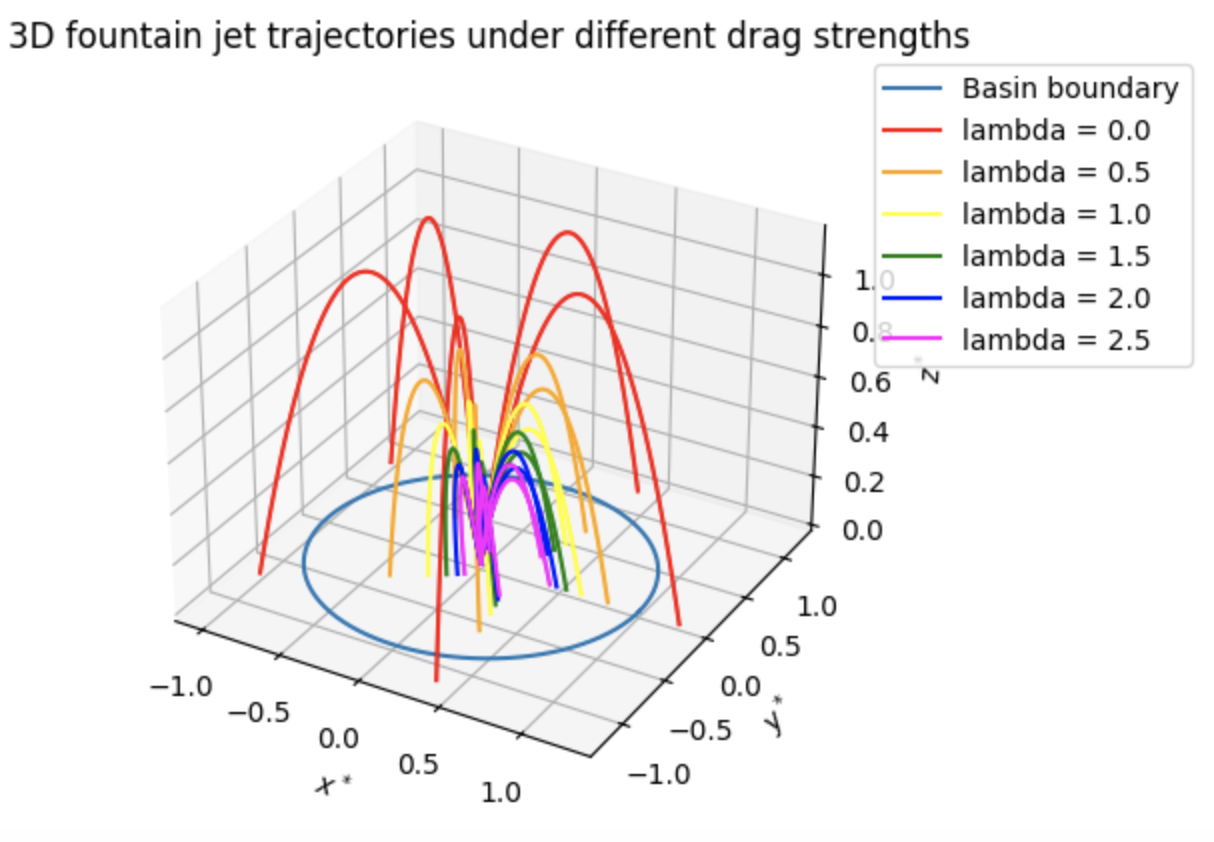
\includegraphics[width=0.47\linewidth]{Figure8.png}
    \caption{3D Fountain Jet Trajectories Under Different Drag Strengths}
    \label{fig:placeholder}
\end{figure}

%\begin{figure} [H]
%    \centering
%    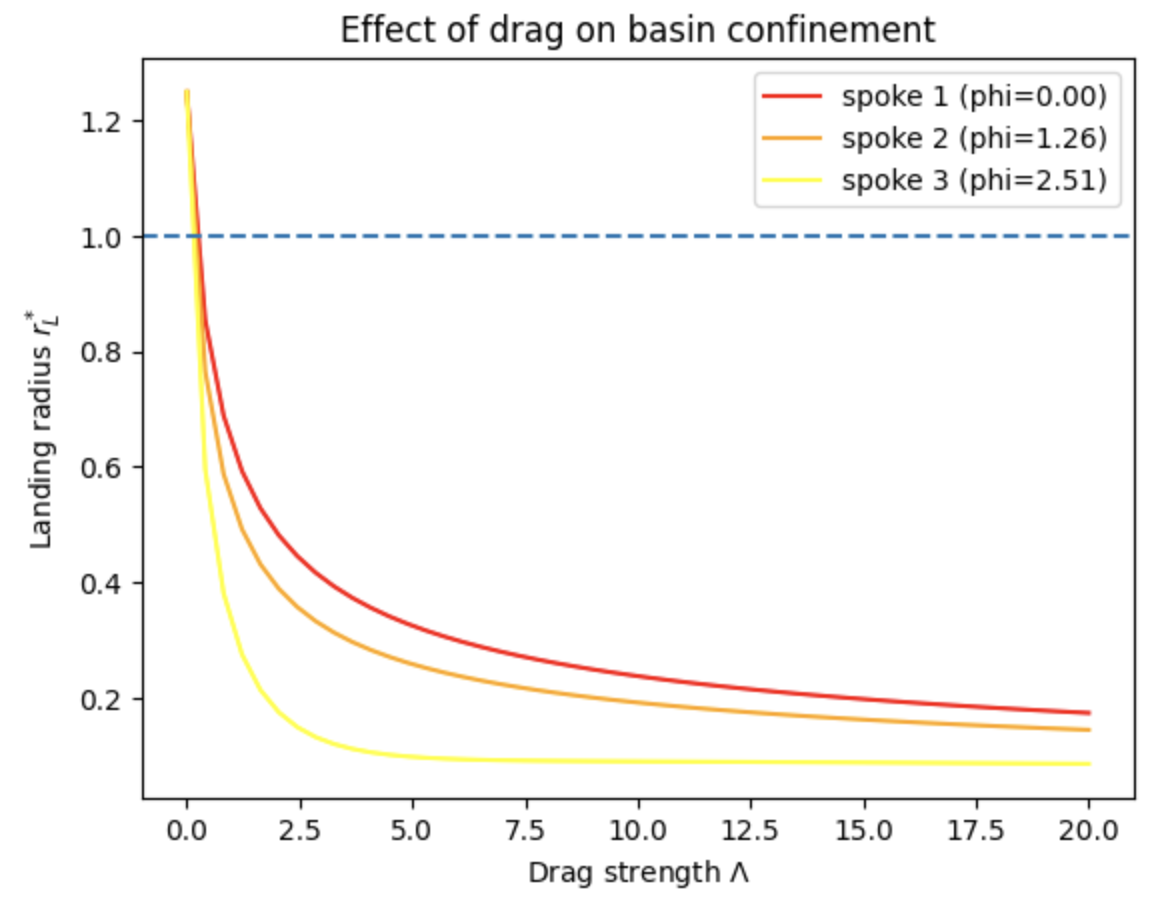
\includegraphics[width=0.5\linewidth]{Figure9.png}
%    \caption{Effect of Drag on Basin Confinement}
%    \label{fig:placeholder}
%\end{figure}

%\begin{figure} [H]
%    \centering
%    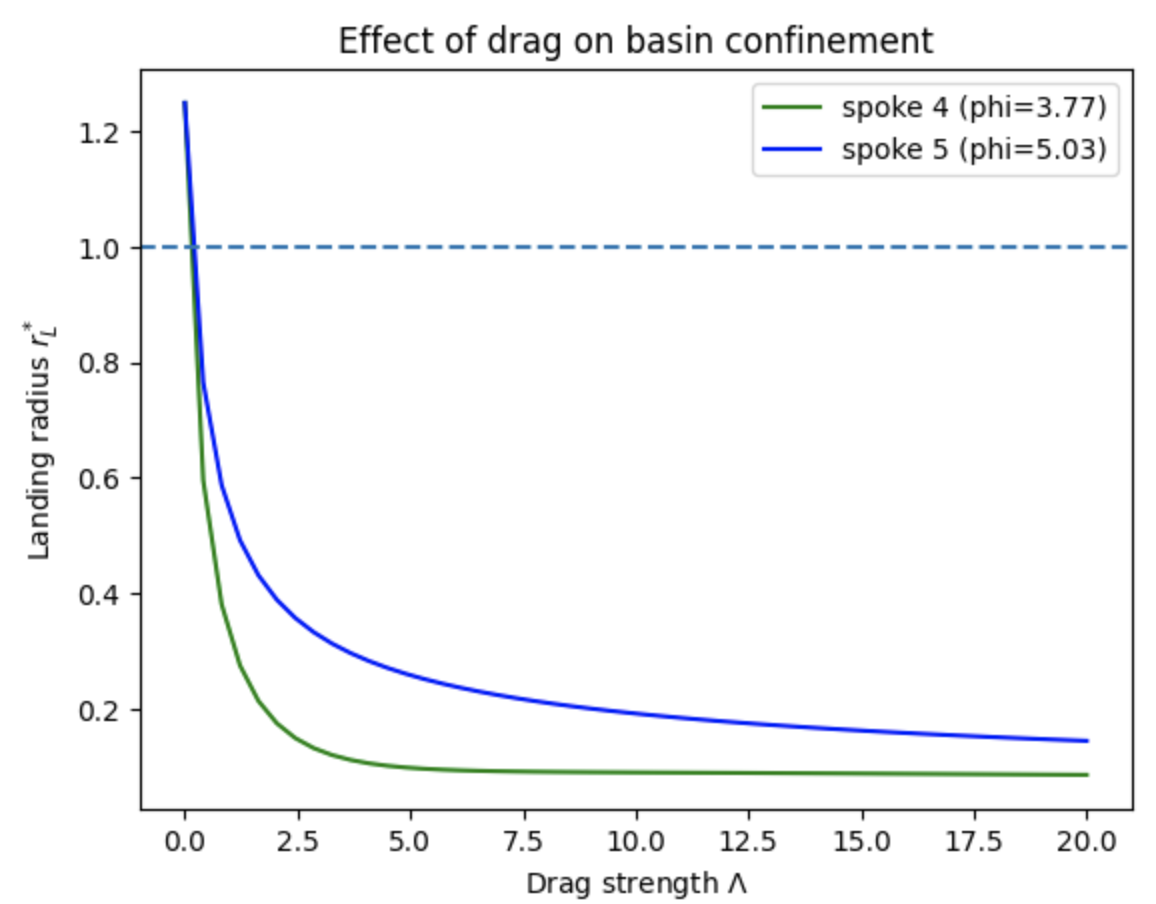
\includegraphics[width=0.5\linewidth]{Figure10.png}
%    \caption{Effect of Drag on Basin Confinement}
%    \label{fig:placeholder}
%\end{figure}

\subsection{Effect of Wind on Required Minimum Radius}

Plotting wind strength vs. minimum basin radius reveals the minimum basin radius required for wind-robust operation for each respective spoke on the nozzle. We see that for any given nozzle, increasing wind strength $u^*$ beyond $1$ requires a minimum fountain basin radius greater than the nominal radius. Increasing wind strengths require increasing minimum basin radii in order to maintain the water trajectories within the basin. This is in accordance with the inverse proportionality relation between drag and horizontal range in projectile motion.


%\begin{figure} [H]
%    \centering
%    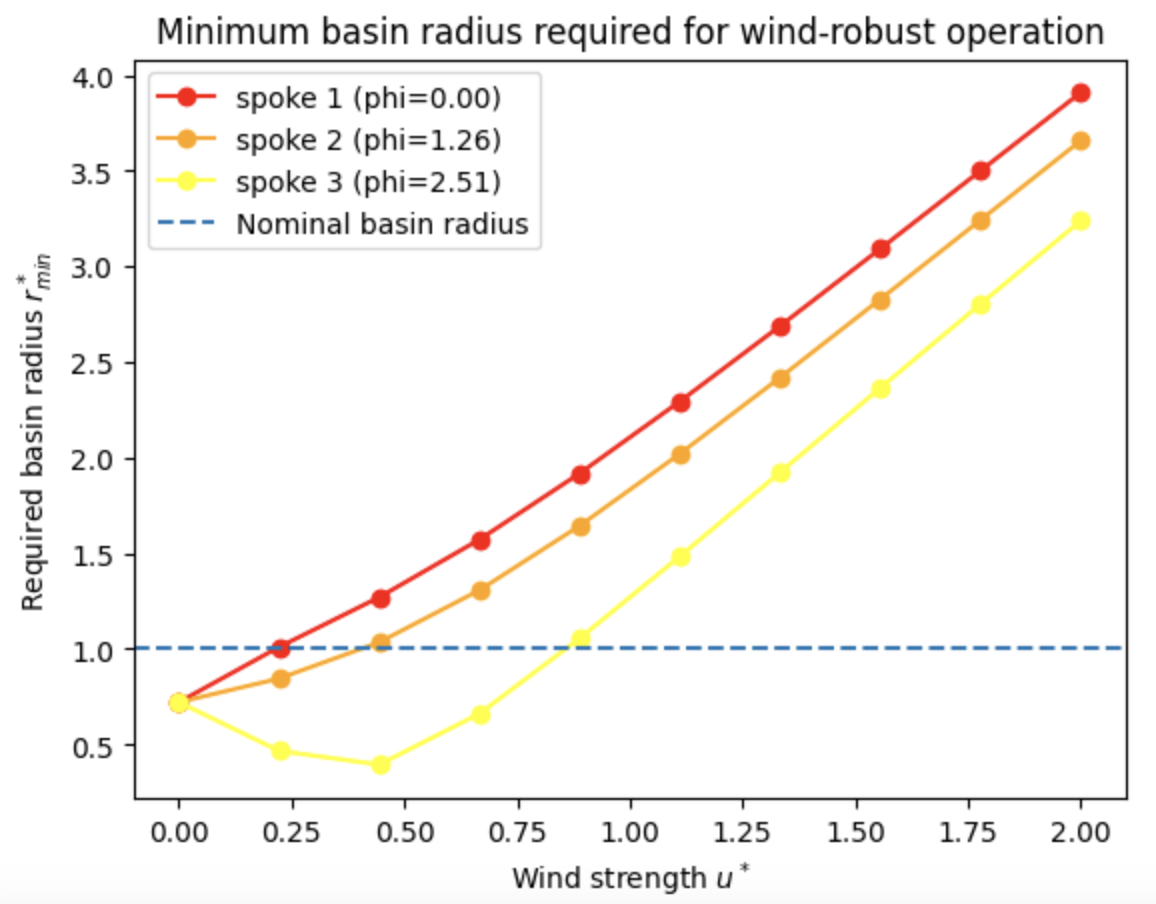
\includegraphics[width=0.5\linewidth]{Figure11.png}
%    \caption{Minimum Basin Radius Required for Wind-Robust Operation}
%    \label{fig:placeholder}
%\end{figure}

%\begin{figure} [H]
%    \centering
%    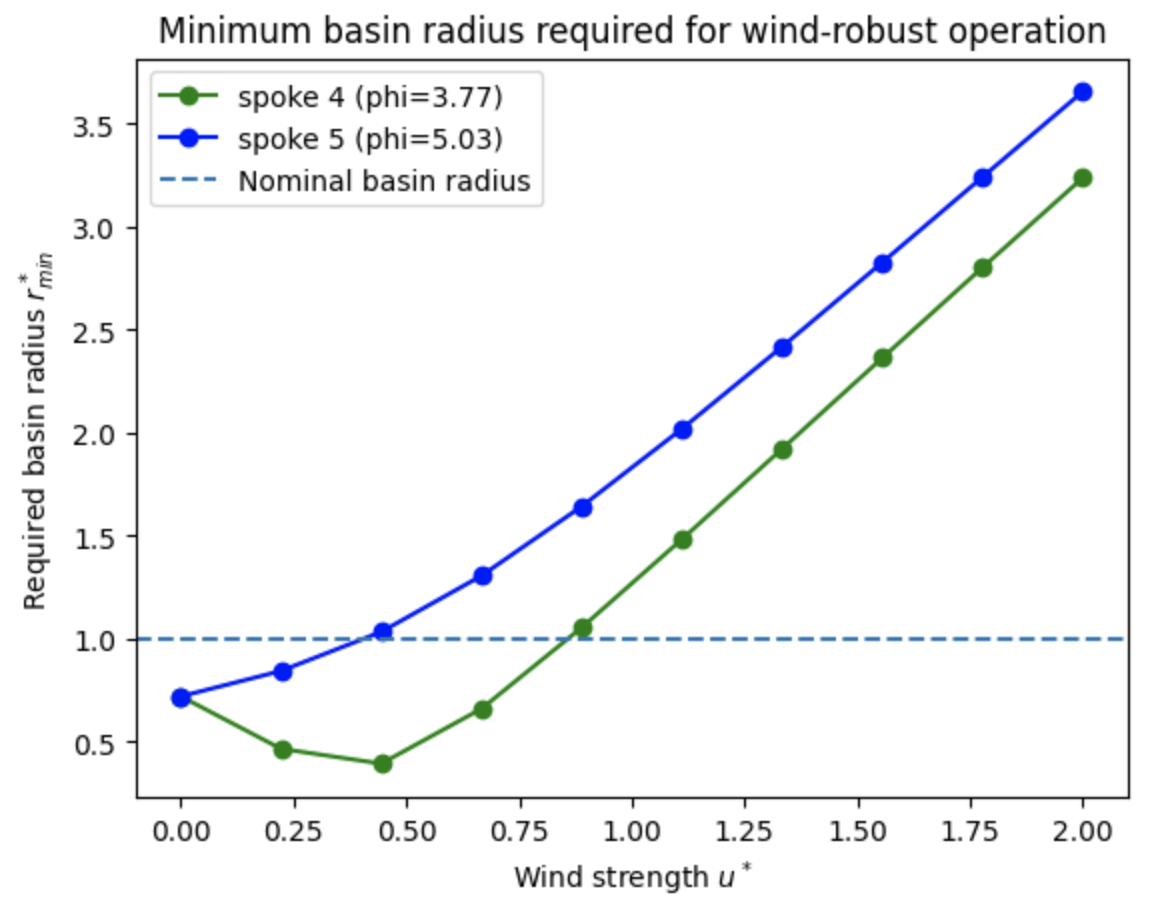
\includegraphics[width=0.5\linewidth]{Figure12.png}
%    \caption{Minimum Basin Radius Required for Wind-Robust Operation}
%    \label{fig:placeholder}
%\end{figure}

\begin{figure}[H]
    \centering
    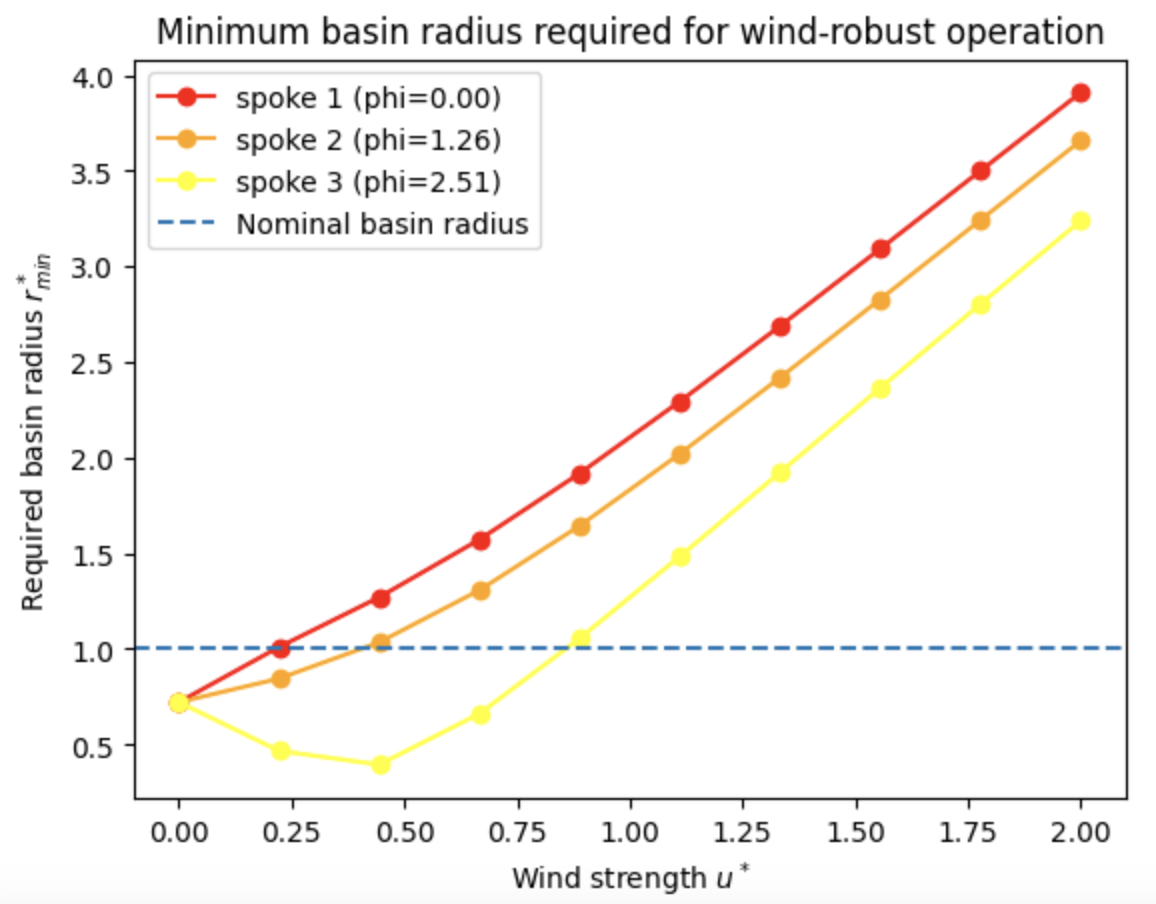
\includegraphics[width=0.45\textwidth]{Figure11.png}
    \hspace{0.5cm}
    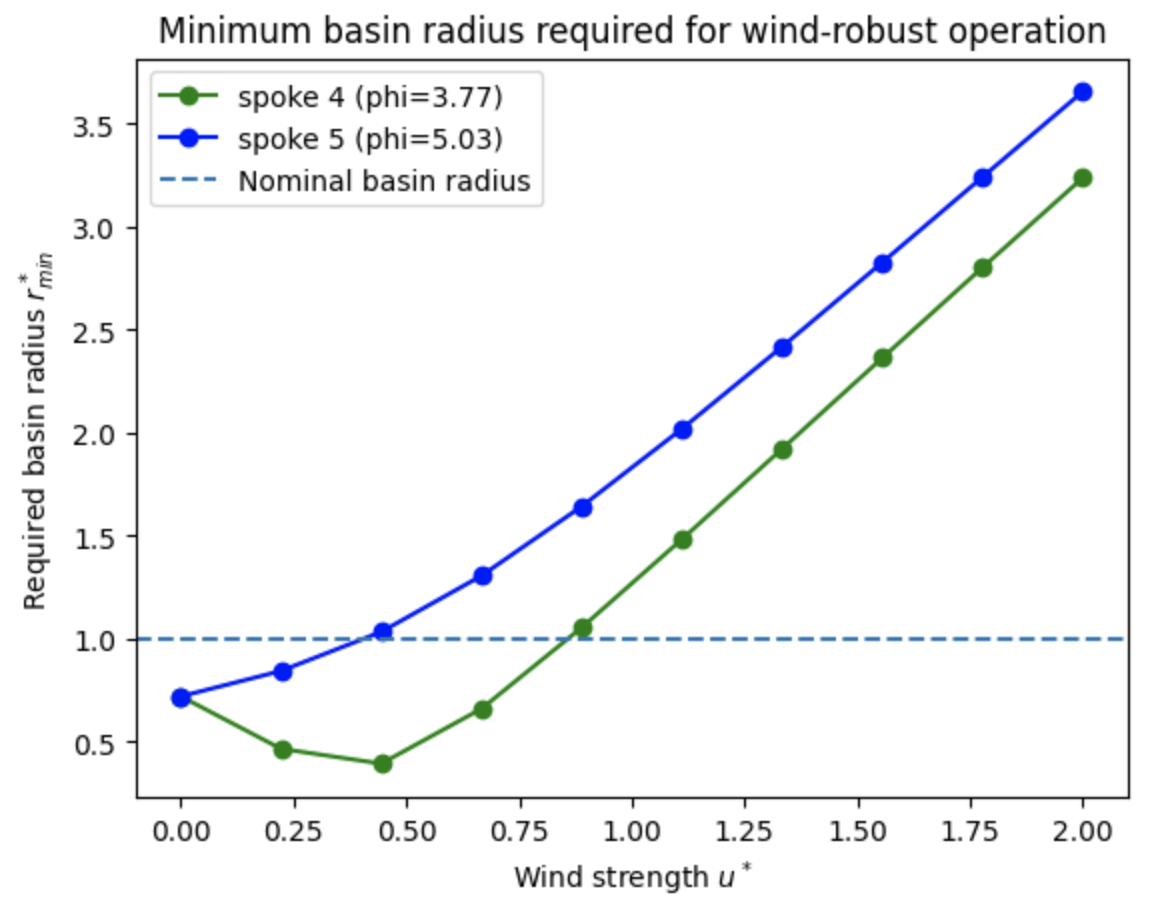
\includegraphics[width=0.45\textwidth]{Figure12.png}
    \caption{Minimum Basin Radius Required for Wind-Robust Operation}
\end{figure}


\subsection{Effect of Wind on Fountain Trajectories}

Plotting fountain trajectories under increasing wind in 3D reveals the effects of wind on the fountain trajectories of each spoke, keeping launch angle and drag constant. We see that for stronger winds, the trajectories skew further in the $x$ direction, with height on the vertical axis decreasing slightly. Plotting the 2D projection on the $x^*-y^*$ plane of the landing locations shows us the precise landing locations for each spoke under a range of wind conditions, with slight overspill beyond the basin boundary.

\begin{figure}[H]
    \centering
    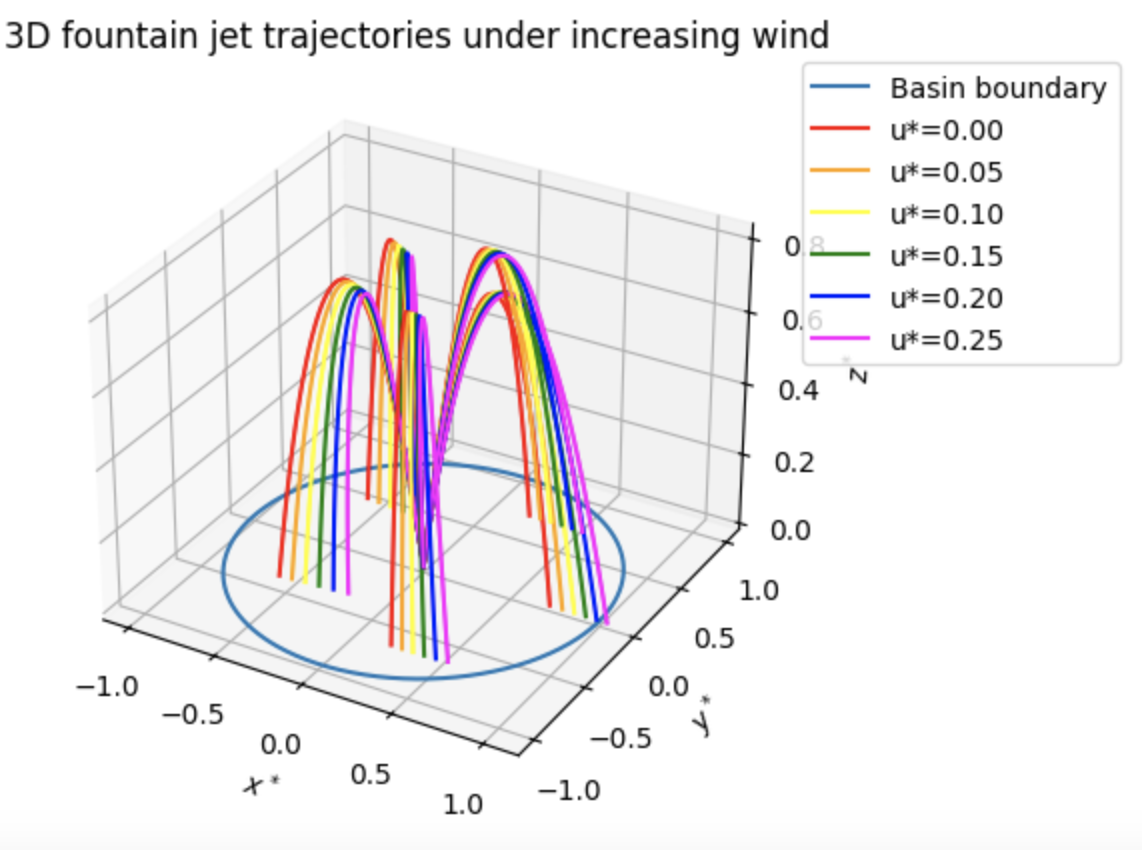
\includegraphics[width=0.47\textwidth]{Figure3.png}
    \hspace{0.5cm}
    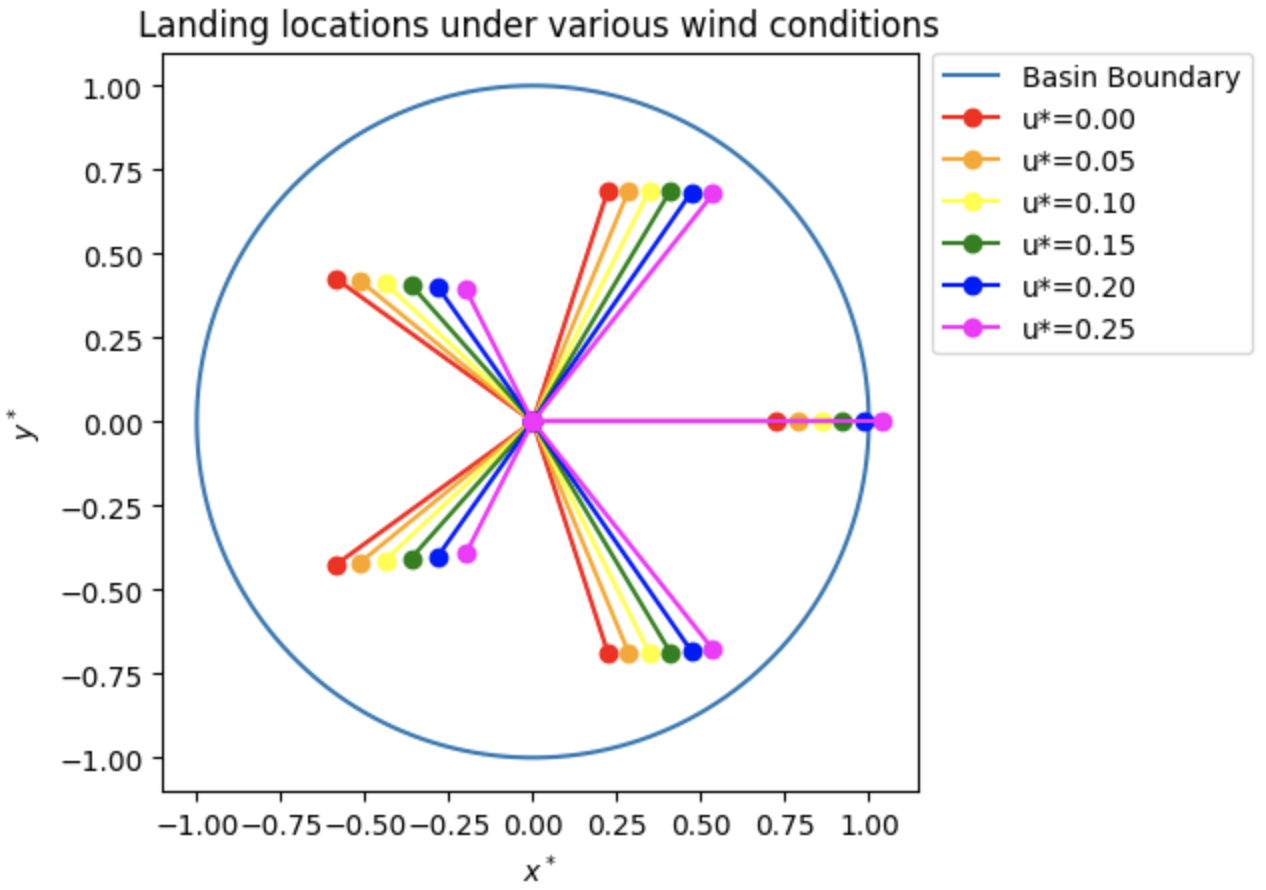
\includegraphics[width=0.47\textwidth]{Figure5.png}
    \caption{Effect of Wind on Fountain Trajectories}
\end{figure}




\section{Conclusion}
Ultimately, our model provides a framework that allows us to model a range of properties of a fountain under select external disturbances, enabling the identification of optimal parameters for the fountain’s functioning and efficiency. By solving the derived nondimensional ODE system and plotting trajectories in two and three dimensions, we deduced the optimal launch angle and drag strength of the fountain, and conducted further investigation of the effects of various wind strengths. This allows us to identify the minimum required basin radius for wind-robust operation of the fountain.

Notwithstanding the various strengths of the presented model, it is important to acknowledge limitations. One such limitation of our model is that we assume constant wind velocity, however, this is unlikely to be the case in practice. This may limit the applicability of our model to a real-world setup, and accounting for non-constant wind velocity may yield different results. Neglecting other effects such as turbulence, evaporation, and splashing also somewhat limits the real-world applicability of the model. We also limited our analysis to a single fountain configuration, which leaves room for further exploration of other designs. Future investigations incorporating the neglected factors in this model as well as other types of fountain designs would be a useful complement to the findings of this model for applications to real-world scenarios.



%Now conclude your report:  summarize your question and key results, in different words. Ask: 
%how would you give a 1-minute summary of the key things you learned, to a peer?
%Explain some limitations of your model, and speculate on directions for further research

\nocite{*}
\bibliographystyle{plain}  % choose style
\bibliography{refs}        % file name WITHOUT .bib


\section*{Gen AI declaration} 

Generative artificial intelligence tools were used in a limited and supportive capacity during the preparation of this report. Specifically, these tools assisted with clarifying background physics concepts related to aerodynamic drag and wind velocity vectors, refining and debugging minor aspects of code used for three-dimensional visualizations, correcting simple programming errors, and improving LaTeX formatting for text and figure alignment.

All scientific reasoning, mathematical modeling, data analysis, interpretation of results, and final conclusions were developed independently by the authors. The use of generative AI did not replace original intellectual contributions, experimental design, or critical evaluation, and the authors take full responsibility for the content of this work.
\end{document}

